\documentclass[../main.tex]{subfiles}

\graphicspath{{\subfix{../imgs/}}}

\begin{document}

\section{Task 7}

In this task, we will use HLS to convert a SystemC hardware description to an RTL implementation.

\begin{itemize}
    \item Write the ADVIOS IP core and a testbench in SystemC.
    \item Document and verify the result of the simulation and synthesis using Vivado HLS.
    \item Connect the ctrl port to the AXI4Lite interface by using pragma as described in UG902, p. 161.
    \item Create a Vivado project and add the ADVIOS IP core and connect it to the LEDS and SWITCHES on the ZYBO board.
    \item Write a program with the Xilinx SDDK that verifies the functionality of the IP core and document the results.
\end{itemize}

\subsection*{Solution}

First we wrote the IP in SystemC for Vivado HLS, according to the specification of the task. 
The IP core has the following interface:

\begin{itemize}
    \item \makebox[1.8cm]{\texttt{ctrl}\hfill}     4-bit input
    \item \makebox[1.8cm]{\texttt{inSwitch}\hfill} 4-bit input
    \item \makebox[1.8cm]{\texttt{outLeds}\hfill}  4-bit output
    \item \makebox[1.8cm]{\texttt{clk}\hfill}      clock signal input
    \item \makebox[1.8cm]{\texttt{reset}\hfill}    reset signal input
\end{itemize}

The advios IP core needs to behave as follows:

\vspace{10pt}
\par
\resizebox{\linewidth}{!}{%
\begin{tabular}{|>{\raggedright}p{3cm}|>{\raggedright\arraybackslash}p{10cm}|}
    \hline
    \textbf{Ctrl value} & \textbf{Behavior} \\
    \hline
    0x0 & The outLeds are incremented by a second counter and cleared by inSwitch. \\
         & \textit{outLeds = increments every 1 second} \\
         & \textit{if inSwitch = 0x8 then clear outLeds} \\
    \hline
    0x1 -- 0xF & The value of outLeds are masked by ctrl register and inSwitch. \\
               & \textit{outLeds = ctrl AND inSwitch} \\
    \hline
\end{tabular}%
}
\vspace{10pt}

To achieve this, we use the clocked threads process in SystemC. The code for the IP core is shown below.
\begin{myminted}{advios.h - SystemC IP Core}
    #include <systemc.h>
    SC_MODULE(advios){
        sc_in<bool> clk;
        sc_in<bool> reset;
        sc_in<sc_uint<4> > inSwitch;
        sc_in<sc_uint<4> > ctrl;
        sc_out<sc_uint<4> > outLeds;
    
        sc_uint<4> switchs;
        sc_uint<4> control;
        sc_uint<28> count;
        sc_uint<4> sec_counter;
        sc_signal<bool> sec_pulse;
    
        void iosThread();
        void countThread();
        SC_CTOR(advios){
            SC_CTHREAD(iosThread, clk.pos());
            reset_signal_is(reset, true);
    
            SC_CTHREAD(countThread, clk.pos());
            reset_signal_is(reset, true);
        }
    };
\end{myminted}
\begin{myminted}{advios.cpp - implementation}
    void advios::iosThread() {
    #pragma HLS RESOURCE variable=ctrl core=AXI4LiteS metadata="-bus_bundle slv0" // pragma for AXI4Lite interface
    
        control = 0x0;
        switchs = 0x0;
        sec_counter = 0x0;
        wait();
    
        while (true) {
            wait(); // Wait for clock event
            control = ctrl.read();
            switchs = inSwitch.read();
    
            switch (control){
                case 0x0:
                    if (switchs == 0x8) {
                        outLeds.write(0x0);
                        sec_counter = 0x0;
                    }else{
                        if(sec_pulse.read()){
        
                            sec_counter++;
                            outLeds.write(sec_counter);
                        }
                    }
                    break;
                default:
                    outLeds.write(control & switchs);
                    break;
            }
        }
    }
    void advios::countThread() {
        wait();
        count = 0;
        while (true) {
            wait();  // Wait for clock event
            count++;
            if (count == 100000000) {
                sec_pulse.write(true);
                count = 0;
            } else {
                sec_pulse.write(false);
            }
        }
    }
\end{myminted}
\newpage
To check if the core is working according to the specification, a testbench was written. The testbench consists of a main code
and a driver module. 
The main declares all signals, module and other components needed for the simulation, and it is also the entry point for the executable. The driver module is designed to test
the different functionalities of the IP core. The testbench driver is shown below:
\begin{myminted}{advios\_driver.cpp - testbench driver}
void advios_driver::test(){
	wait();
	reset.write(true); //test reset signal
	ctrl.write(0x0);
	outSwitch.write(0x0);
	wait_c(3); //wait for 3 clock cycles
	reset.write(false);
	wait();

	sc_uint<4> leds_result; //test ctrl AND switch (when ctrl = 0x1-0xF)
	bool mask_result = true;
	for (sc_uint<4> i_ctrl = 0x1; i_ctrl < 0xF; i_ctrl++) {
	    for (sc_uint<4> i_outSwitch = 0x0; i_outSwitch < 0xF; i_outSwitch++) {
	        ctrl.write(i_ctrl);
	        outSwitch.write(i_outSwitch);
	        wait_c(2);  // Wait for two clock cycles to allow signal propagation
	        leds_result = inLeds.read();
	        if (!(leds_result == (i_outSwitch & i_ctrl))) { //check if the output is correct
	            mask_result = false; //if not, test has failed
	        }
	    }
	}

	wait_c(10); //wait for 10 clock cycles
	ctrl.write(0x0);
	reset.write(true);
	wait();
	reset.write(false);
	for(sc_uint<4> i_outSwitch = 0x0; i_outSwitch < 0xf; i_outSwitch++){ //test counter
		outSwitch.write(i_outSwitch);
		for (int i = 0; i < 16; i++){
			wait();
		}
	}
}
\end{myminted}
\newpage
The testbench was simulated in Vivado HLS. First we did a C simulation, and then a C/RTL co-simulation. The first two figures shows the results of the C simulation.
For the simulation the IP core counter was set to generate a pulse for every two clocks. 
\begin{figure}[h]
    \centering
    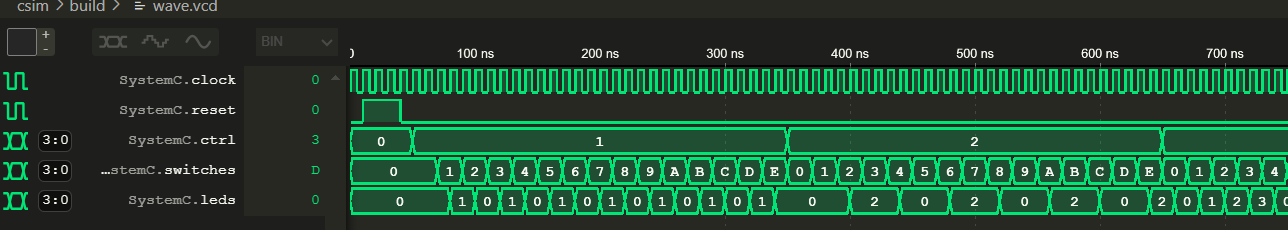
\includegraphics[width=1\textwidth]{csim-ctrl-0x1-0xf.png}
    \caption{C-simulation of the IP core with ctrl set to 0x1-0xF}
\end{figure}

\begin{figure}[h]
    \centering
    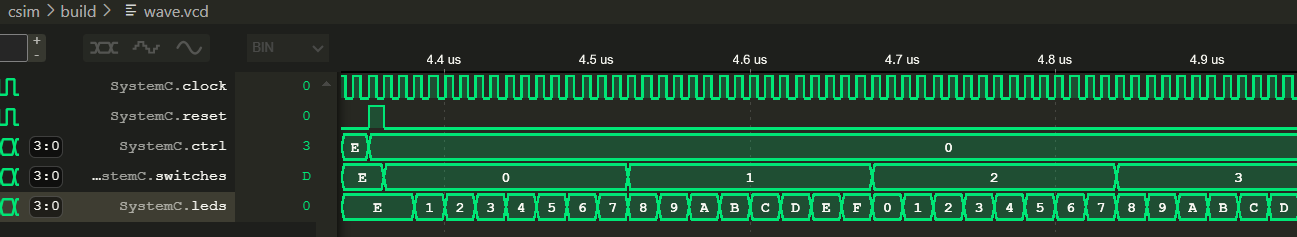
\includegraphics[width=1\textwidth]{csim-ctrl-0x0.png}
    \caption{C-simulation of the IP core with ctrl set to 0x0}
\end{figure}
\par
The waveform of the C simulation shows that the IP core is working as expected.

\begin{figure}[h]
    \centering
    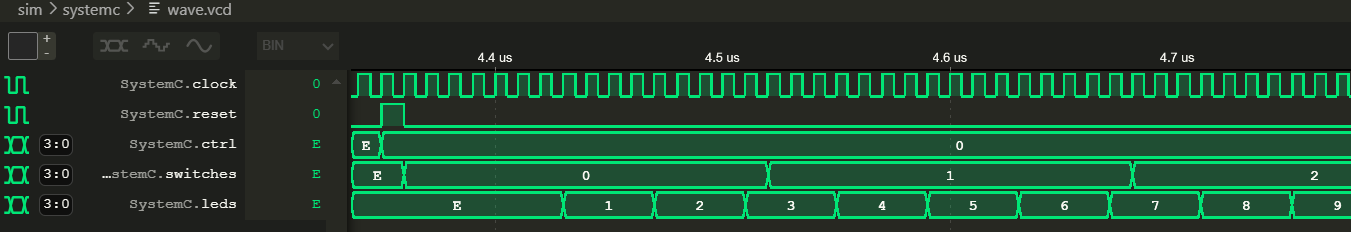
\includegraphics[width=1\textwidth]{syn-sim-sysc-ctrl-0x0.png}
    \caption{C/RTL simulation of the IP core with ctrl set to 0x0}
\end{figure}

The C/RTL co-simulation showed a different result. The IP core did not behave as in the C-simulation in the pulse generation. 
The simulation showed that the code execution could not be completed within the clock cycle, resulting in a pulse generation half the speed of the C-simulation.

\newpage

We had the \textit{classic} of issue of Vivado not wanting to generate the necessary files for the IP core in the BSP. To read/write to the IP core register, we chose to simply use \texttt{Xil\_Out8}. We found the driver file of the IP core, and looked up the register offset to be \texttt{0x14}. A test program was written where different values could be written to the \texttt{ctrl} register. In addition we also added to capability to read the value of the register. The main event loop of the program is shown below.

\begin{myminted}{main.c - Main Event Loop}
while (1)
{
    xil_printf("\r\n\nCMD:> ");
    input = inbyte();
    xil_printf("%c", input);
    switch (input)
    {
        case '0':
            xil_printf("\r\nReading CTRL: ");
            ctrl_read = Xil_In8(CTRL_ADDR) & 0xF;
            xil_printf("%u", ctrl_read);
            break;
        case '1':
            xil_printf("\r\nWriting 0x0 to CTRL.");
            Xil_Out8(CTRL_ADDR, 0x0);
            break;
        case '2':
            xil_printf("\r\nWriting 0xA to CTRL.");
            Xil_Out8(CTRL_ADDR, 0xA);
            break;
        case '3':
            xil_printf("\r\nWriting 0xF to CTRL.");
            Xil_Out8(CTRL_ADDR, 0xF);
            break;
        case '4':
            xil_printf("\r\nGenerating random value.");
            uint8_t rand = rand_uint8() & 0xF;
            xil_printf("\r\nWriting %u to CTRL.", rand);
            Xil_Out8(CTRL_ADDR, rand);
            break;
        default:
            xil_printf("\r\nUnrecognized input. \"%c\"", input);
            break;
    }
}
\end{myminted}

In conclusion our Advios IP core \textit{mostly} works as expected. As noted before, the C/RTL co-simulation showed that the timer was counting at half the intended speed, and that was also observed when running the IP core on the ZYBO board. Aside from that, the IP core works as intended.

\end{document}